\appendix

% =============================================================================
\chapter{Résultats détaillés de la classification des stades}
\label{annexe:staging}
% =============================================================================

Cette annexe rassemble l'intégralité des résultats produits par les douze modèles de
base et les quatre ensembles. Les figures représentatives commentées dans le
chapitre~\ref{chap:realisation-ia} en sont extraites.

Rappel de la convention de dénomination : \texttt{ARCH\_Nch\_Kcls} désigne
l'architecture \texttt{ARCH} entraînée sur \texttt{N} dérivations pour une
classification en \texttt{K} stades.

% -----------------------------------------------------------------------------
\section{Courbes d'apprentissage des douze modèles}
% -----------------------------------------------------------------------------

Chaque figure présente, sur les trente époques d'entraînement, l'évolution de la
perte, de l'exactitude et du $\kappa$ de Cohen évalué sur l'ensemble de validation.
La ligne horizontale en pointillés marque le meilleur $\kappa$ atteint, qui détermine
le point de contrôle retenu.

\subsection{Architecture convolutive}

\begin{figure}[H]
\centering
\begin{subfigure}{\textwidth}
  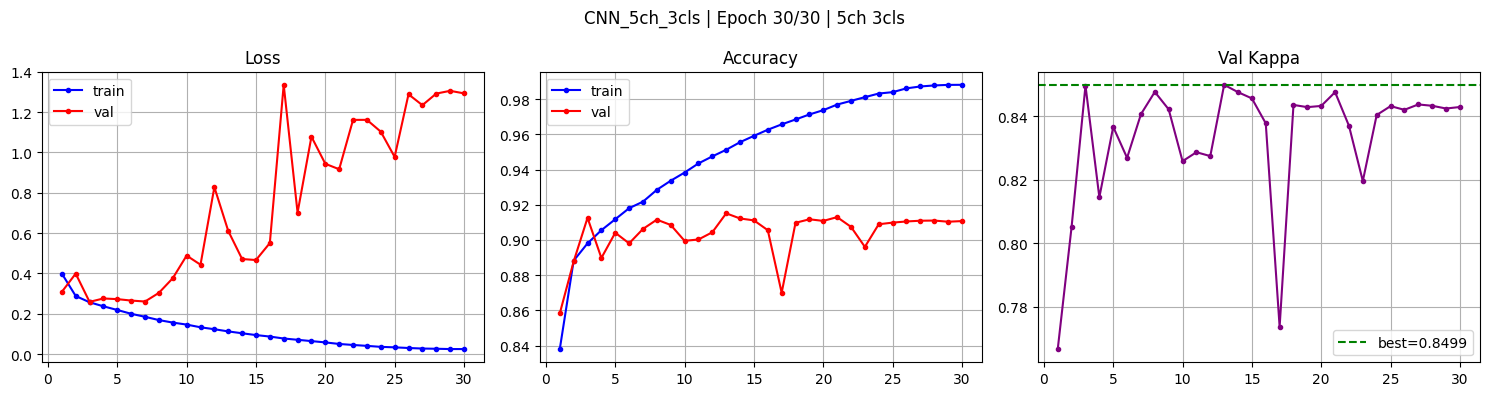
\includegraphics[width=\linewidth]{images/resultats/curves_CNN_5ch_3cls.png}
  \caption{5 dérivations, 3 classes}
\end{subfigure}\\[6pt]
\begin{subfigure}{\textwidth}
  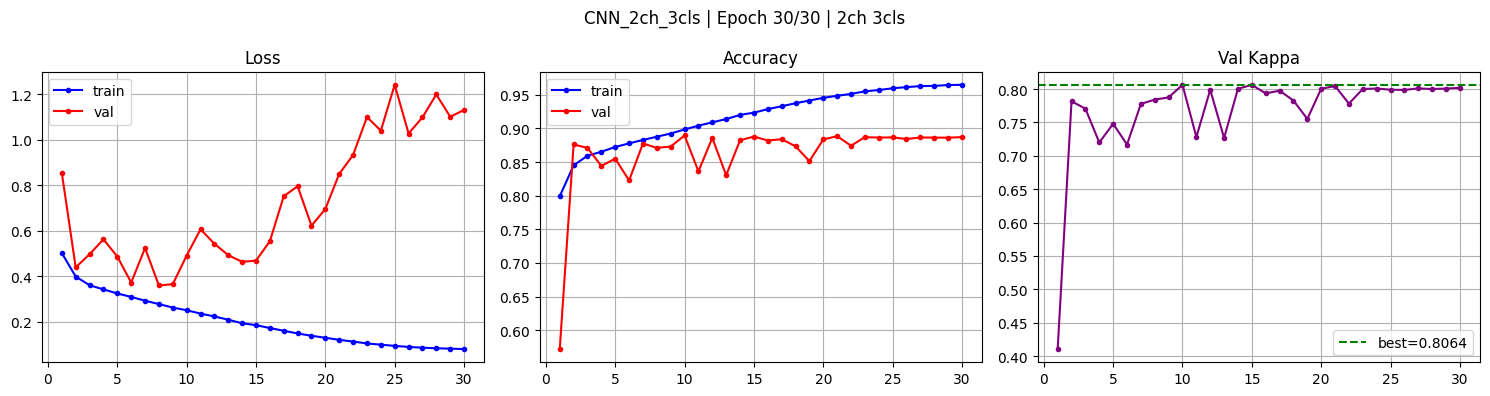
\includegraphics[width=\linewidth]{images/resultats/curves_CNN_2ch_3cls.png}
  \caption{2 dérivations, 3 classes}
\end{subfigure}\\[6pt]
\begin{subfigure}{\textwidth}
  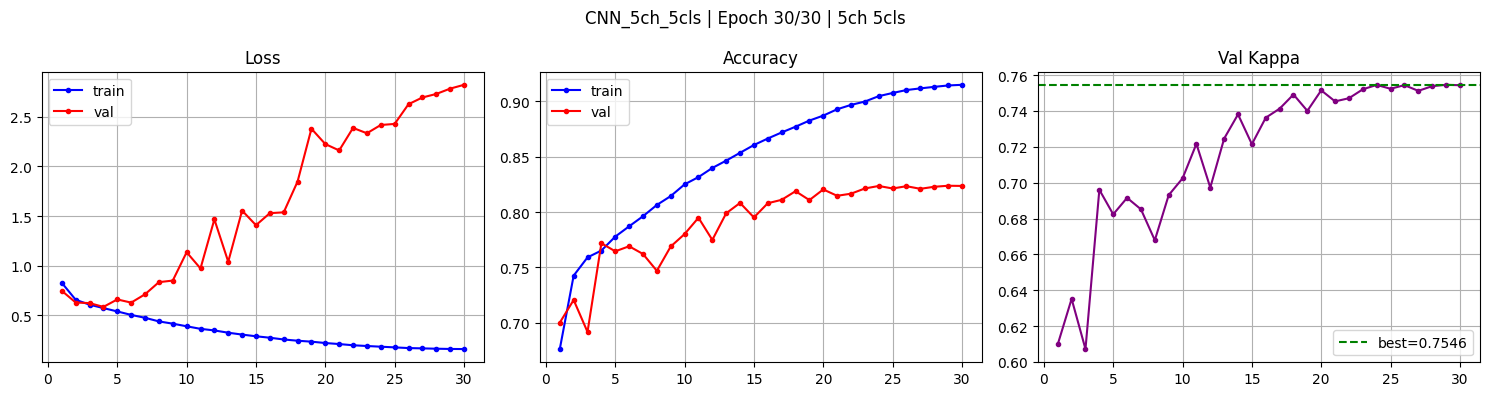
\includegraphics[width=\linewidth]{images/resultats/curves_CNN_5ch_5cls.png}
  \caption{5 dérivations, 5 classes}
\end{subfigure}\\[6pt]
\begin{subfigure}{\textwidth}
  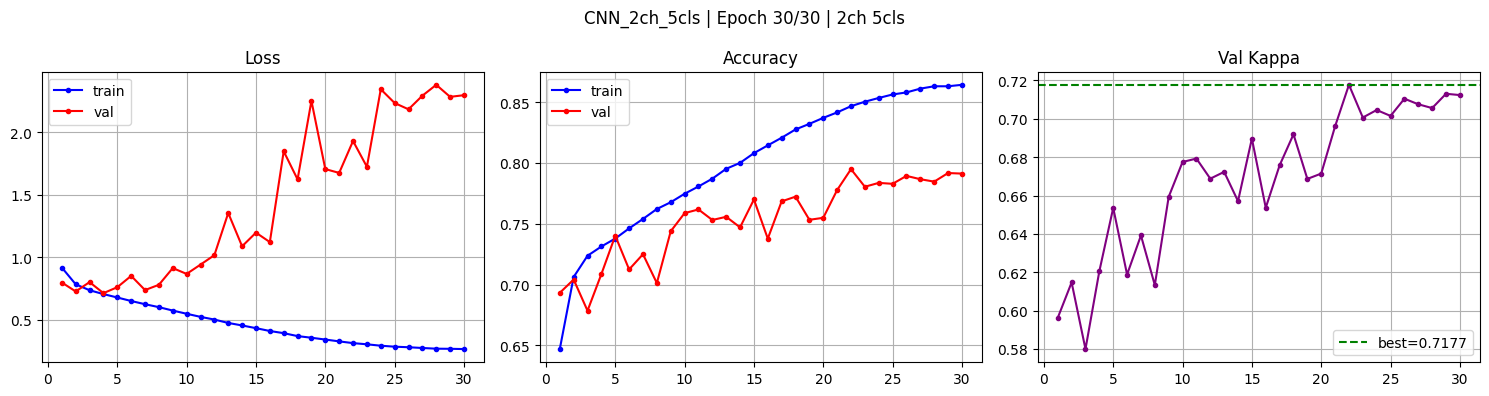
\includegraphics[width=\linewidth]{images/resultats/curves_CNN_2ch_5cls.png}
  \caption{2 dérivations, 5 classes}
\end{subfigure}
\caption[Courbes d'apprentissage --- architecture convolutive]%
        {Courbes d'apprentissage des quatre variantes de l'architecture convolutive.}
\label{fig:ann-curves-cnn}
\end{figure}

\clearpage
\subsection{Architecture récurrente}

\begin{figure}[H]
\centering
\begin{subfigure}{\textwidth}
  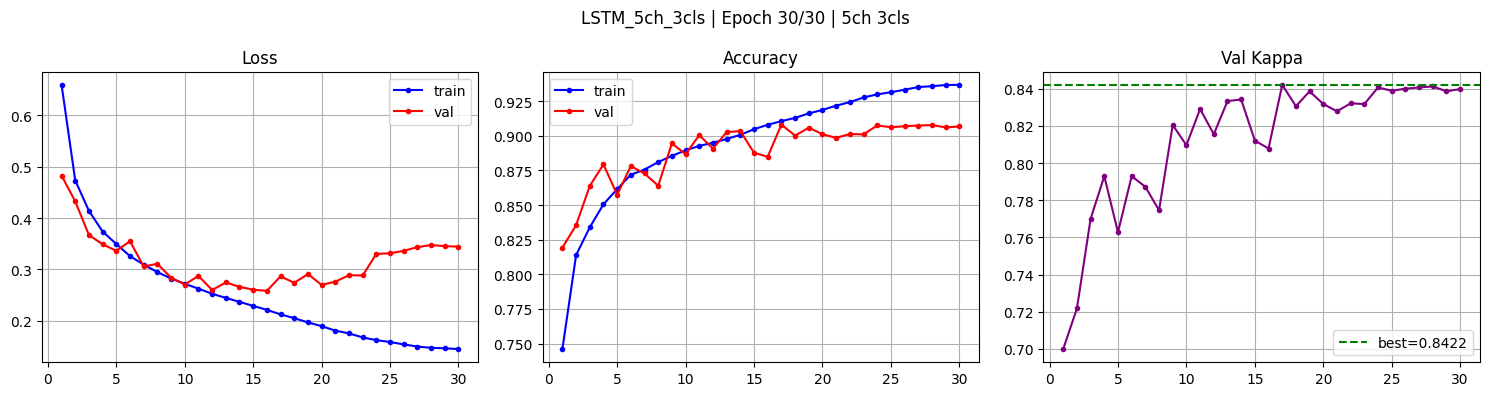
\includegraphics[width=\linewidth]{images/resultats/curves_LSTM_5ch_3cls.png}
  \caption{5 dérivations, 3 classes}
\end{subfigure}\\[6pt]
\begin{subfigure}{\textwidth}
  
\includegraphics[width=\linewidth]{images/resultats/curves_LSTM_2ch_3cls.png}
  \caption{2 dérivations, 3 classes}
\end{subfigure}\\[6pt]
\begin{subfigure}{\textwidth}
  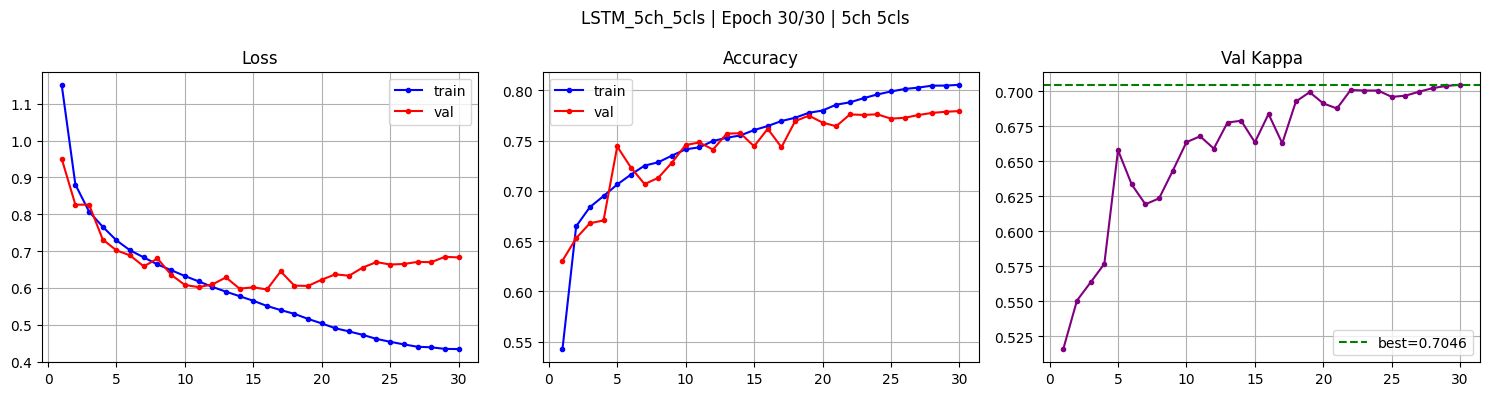
\includegraphics[width=\linewidth]{images/resultats/curves_LSTM_5ch_5cls.png}
  \caption{5 dérivations, 5 classes}
\end{subfigure}\\[6pt]
\begin{subfigure}{\textwidth}
  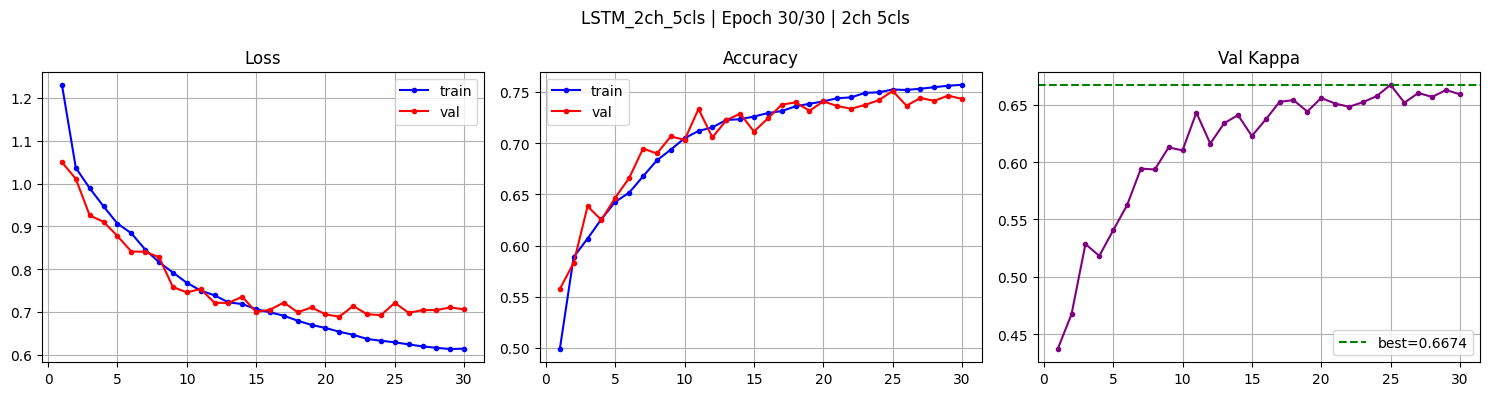
\includegraphics[width=\linewidth]{images/resultats/curves_LSTM_2ch_5cls.png}
  \caption{2 dérivations, 5 classes}
\end{subfigure}
\caption[Courbes d'apprentissage --- architecture récurrente]%
        {Courbes d'apprentissage des quatre variantes de l'architecture récurrente.}
\label{fig:ann-curves-lstm}
\end{figure}

\clearpage
\subsection{Architecture attentionnelle}

\begin{figure}[H]
\centering
\begin{subfigure}{\textwidth}
  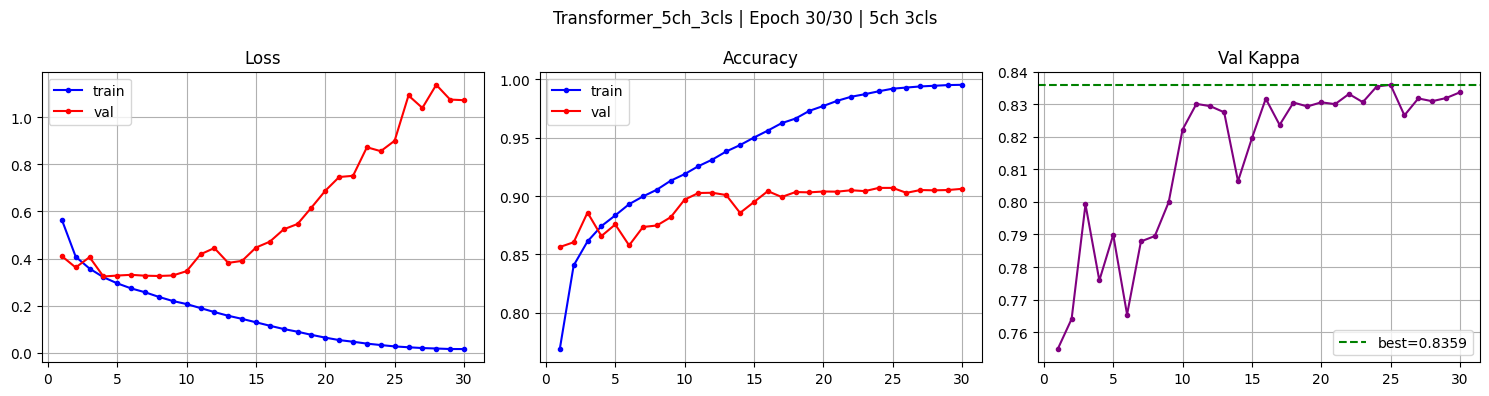
\includegraphics[width=\linewidth]{images/resultats/curves_Transformer_5ch_3cls.png}
  \caption{5 dérivations, 3 classes --- variante réduite à 150 sujets}
\end{subfigure}\\[6pt]
\begin{subfigure}{\textwidth}
  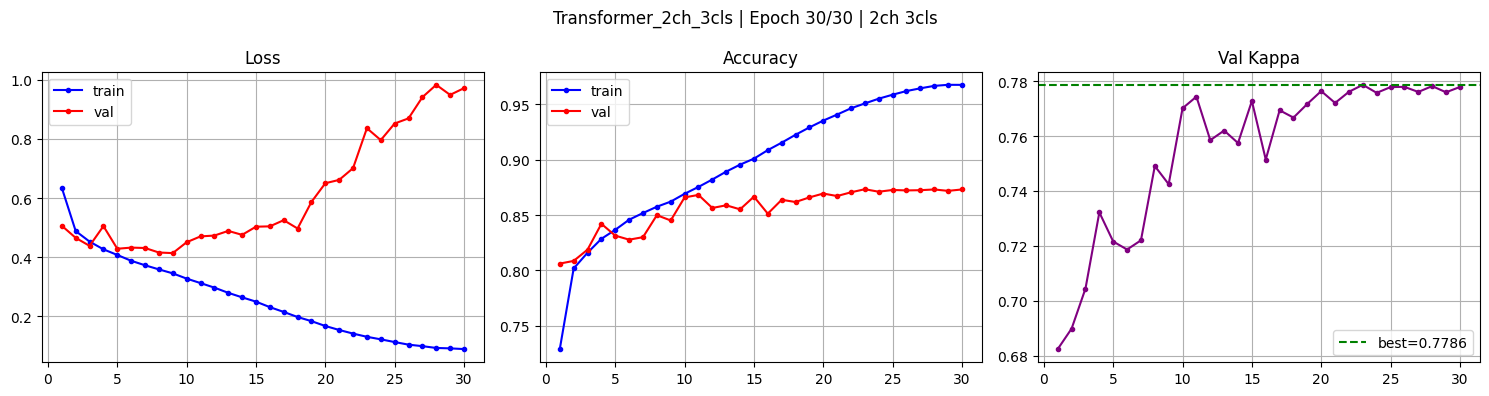
\includegraphics[width=\linewidth]{images/resultats/curves_Transformer_2ch_3cls.png}
  \caption{2 dérivations, 3 classes}
\end{subfigure}\\[6pt]
\begin{subfigure}{\textwidth}
  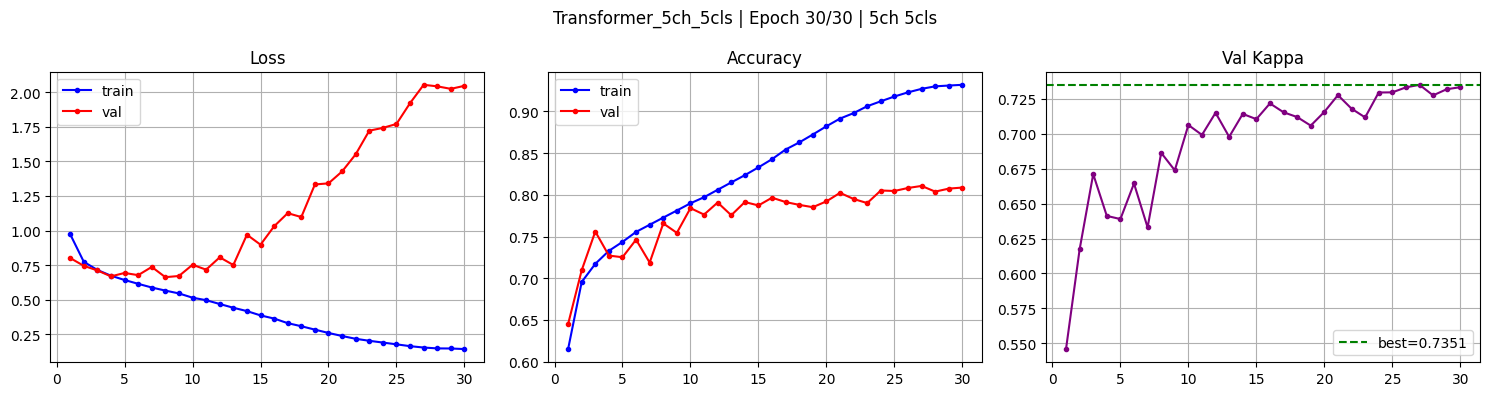
\includegraphics[width=\linewidth]{images/resultats/curves_Transformer_5ch_5cls.png}
  \caption{5 dérivations, 5 classes}
\end{subfigure}\\[6pt]
\begin{subfigure}{\textwidth}
  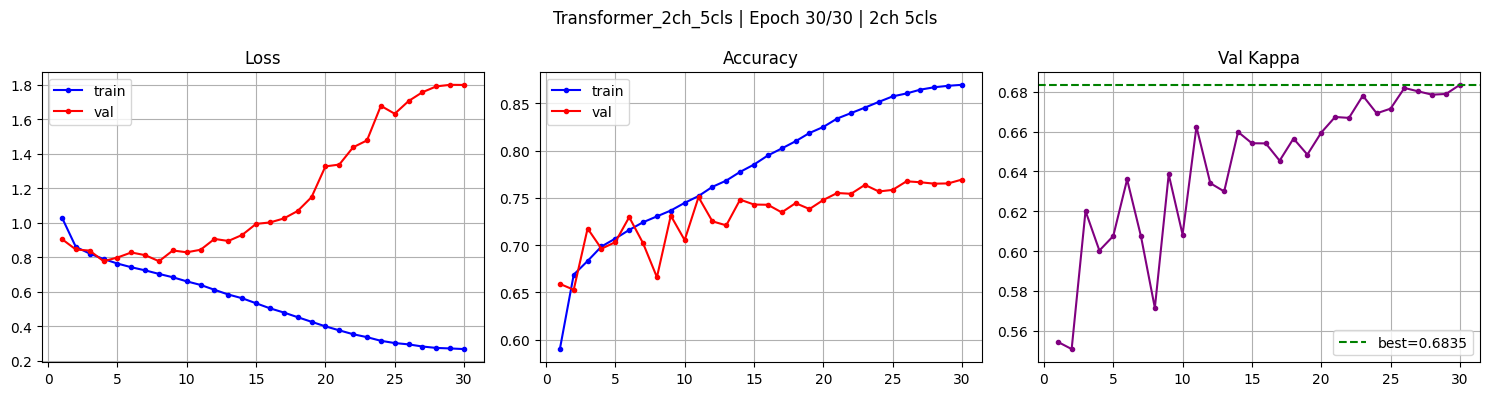
\includegraphics[width=\linewidth]{images/resultats/curves_Transformer_2ch_5cls.png}
  \caption{2 dérivations, 5 classes}
\end{subfigure}
\caption[Courbes d'apprentissage --- architecture attentionnelle]%
        {Courbes d'apprentissage des quatre variantes de l'architecture attentionnelle.}
\label{fig:ann-curves-transformer}
\end{figure}

\clearpage
% -----------------------------------------------------------------------------
\section{Matrices de confusion des douze modèles}
% -----------------------------------------------------------------------------

Les matrices donnent les effectifs bruts sur le jeu de test, soit \num{19513} époques
pour l'ensemble des variantes à l'exception du modèle attentionnel à cinq dérivations
et trois classes, qui en compte \num{14896} pour la raison exposée à la
section~\ref{sec:strategie}.

\subsection{Classification en trois stades}

\begin{figure}[H]
\centering
\begin{subfigure}[t]{0.48\textwidth}
  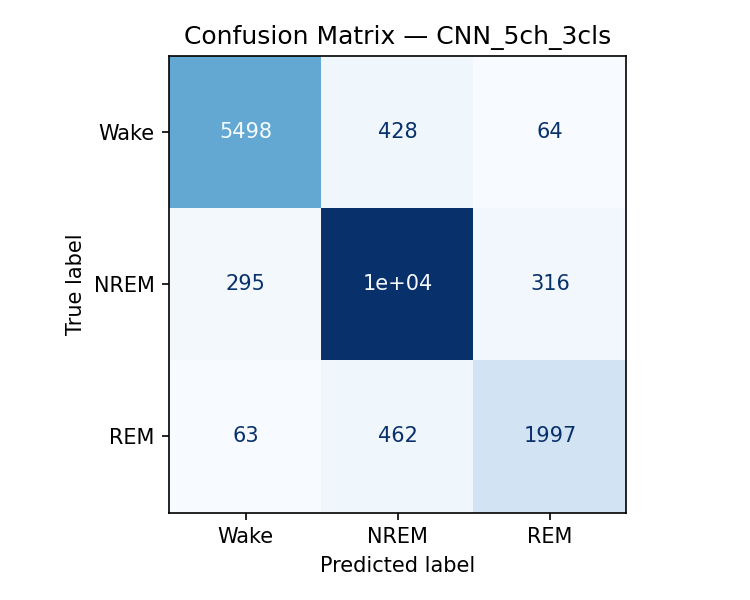
\includegraphics[width=\linewidth]{images/resultats/cm_CNN_5ch_3cls.png}
  \caption{Convolutif, 5 dérivations}
\end{subfigure}\hfill
\begin{subfigure}[t]{0.48\textwidth}
  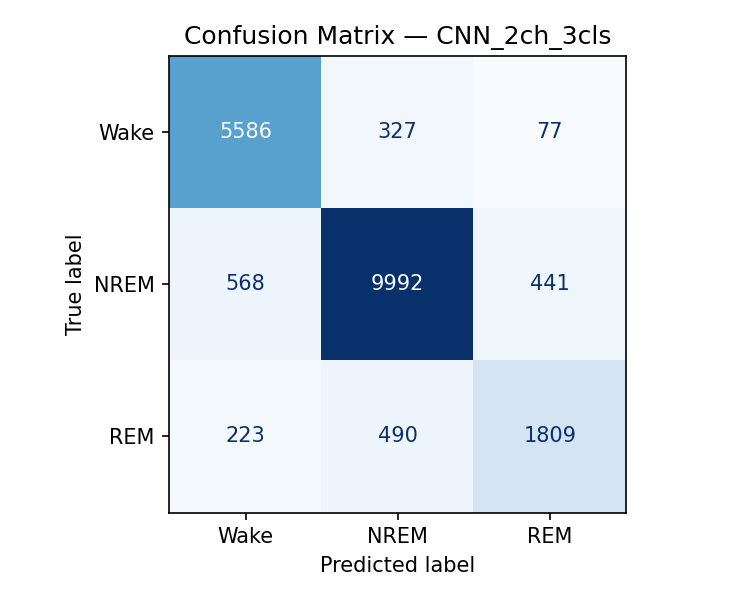
\includegraphics[width=\linewidth]{images/resultats/cm_CNN_2ch_3cls.png}
  \caption{Convolutif, 2 dérivations}
\end{subfigure}\\[8pt]
\begin{subfigure}[t]{0.48\textwidth}
  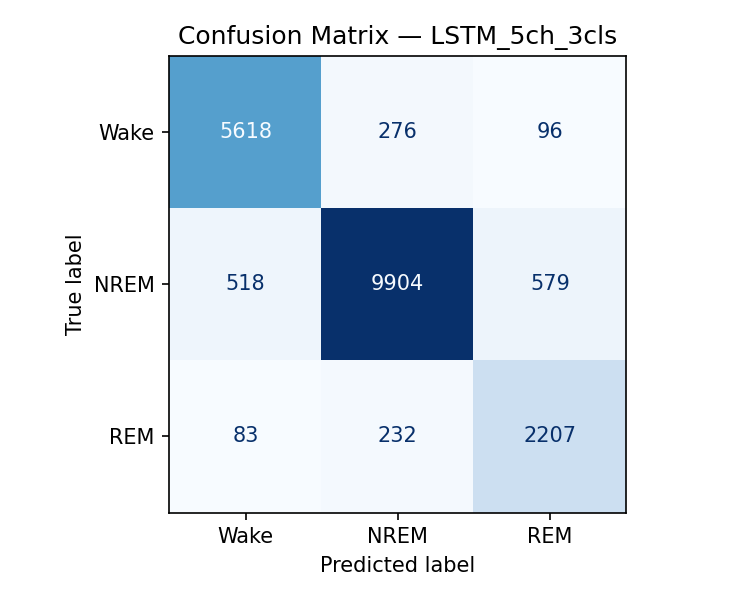
\includegraphics[width=\linewidth]{images/resultats/cm_LSTM_5ch_3cls.png}
  \caption{Récurrent, 5 dérivations}
\end{subfigure}\hfill
\begin{subfigure}[t]{0.48\textwidth}
  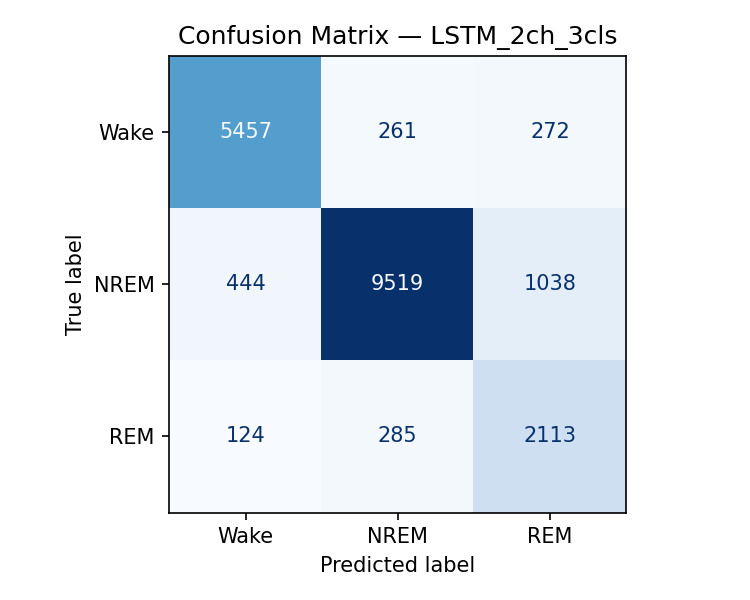
\includegraphics[width=\linewidth]{images/resultats/cm_LSTM_2ch_3cls.png}
  \caption{Récurrent, 2 dérivations}
\end{subfigure}\\[8pt]
\begin{subfigure}[t]{0.48\textwidth}
  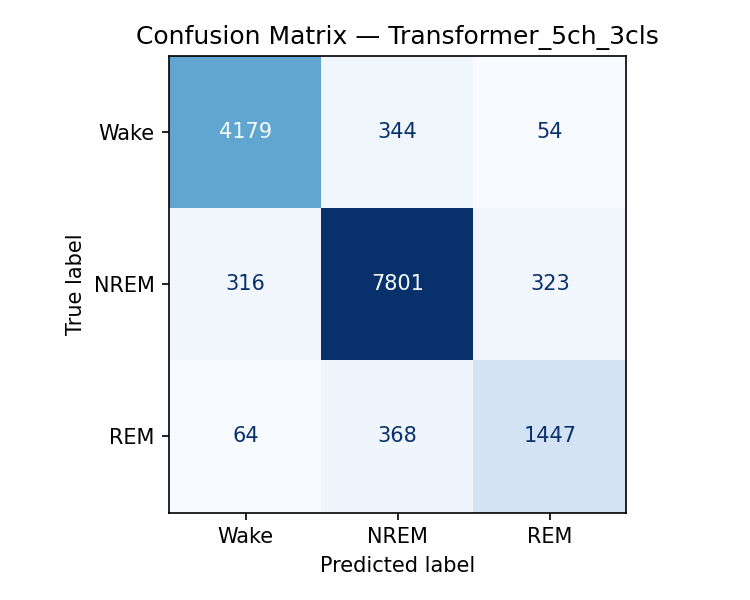
\includegraphics[width=\linewidth]{images/resultats/cm_Transformer_5ch_3cls.png}
  \caption{Attentionnel, 5 dérivations}
\end{subfigure}\hfill
\begin{subfigure}[t]{0.48\textwidth}
  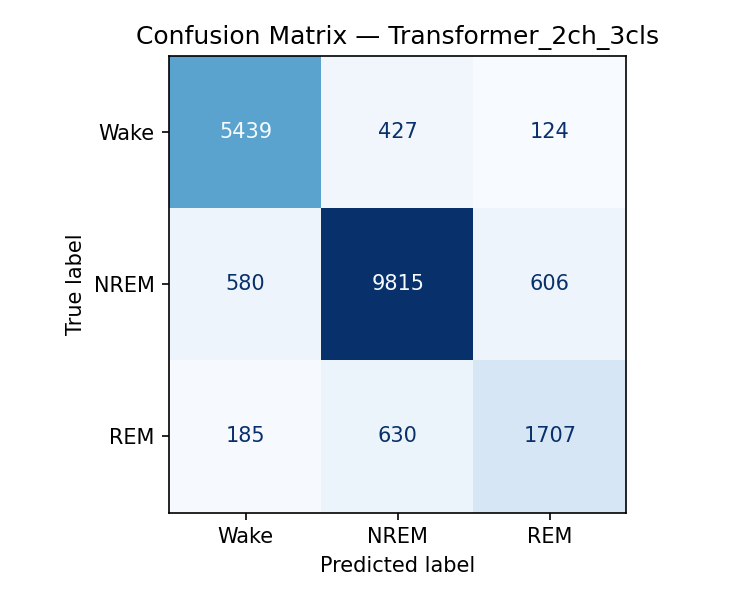
\includegraphics[width=\linewidth]{images/resultats/cm_Transformer_2ch_3cls.png}
  \caption{Attentionnel, 2 dérivations}
\end{subfigure}
\caption[Matrices de confusion --- classification en trois stades]%
        {Matrices de confusion des six modèles de classification en trois stades.}
\label{fig:ann-cm-3cls}
\end{figure}

\clearpage
\subsection{Classification en cinq stades}

\begin{figure}[H]
\centering
\begin{subfigure}[t]{0.48\textwidth}
  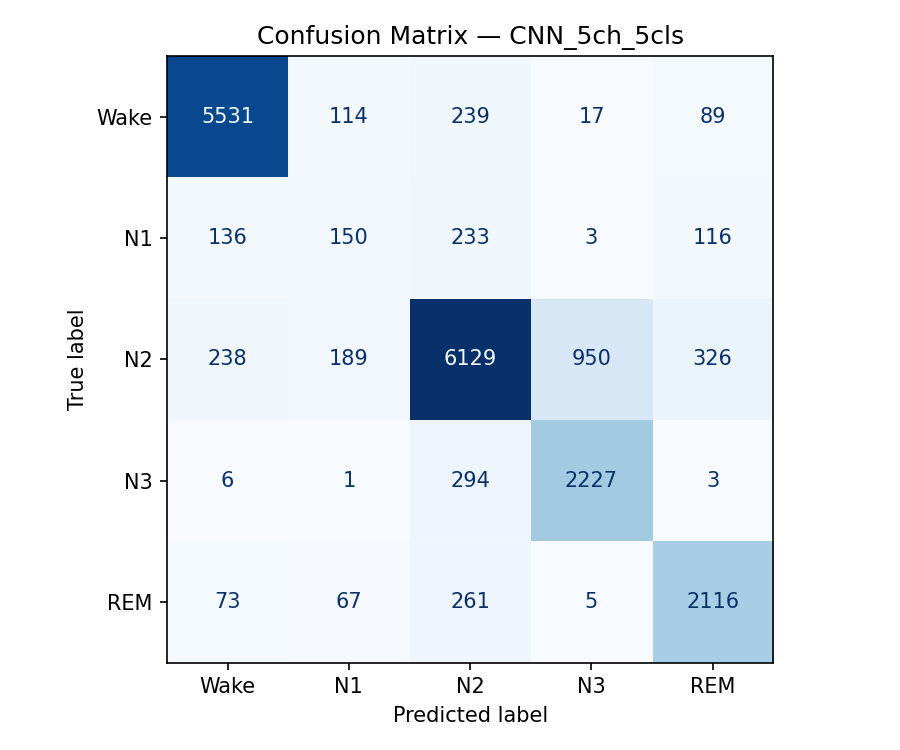
\includegraphics[width=\linewidth]{images/resultats/cm_CNN_5ch_5cls.png}
  \caption{Convolutif, 5 dérivations}
\end{subfigure}\hfill
\begin{subfigure}[t]{0.48\textwidth}
  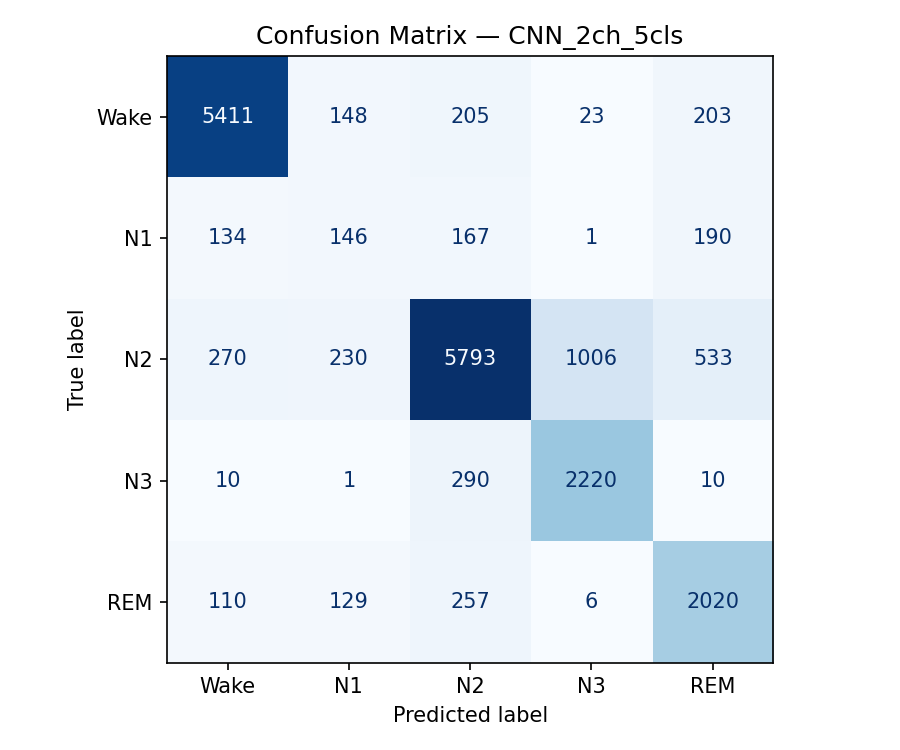
\includegraphics[width=\linewidth]{images/resultats/cm_CNN_2ch_5cls.png}
  \caption{Convolutif, 2 dérivations}
\end{subfigure}\\[8pt]
\begin{subfigure}[t]{0.48\textwidth}
  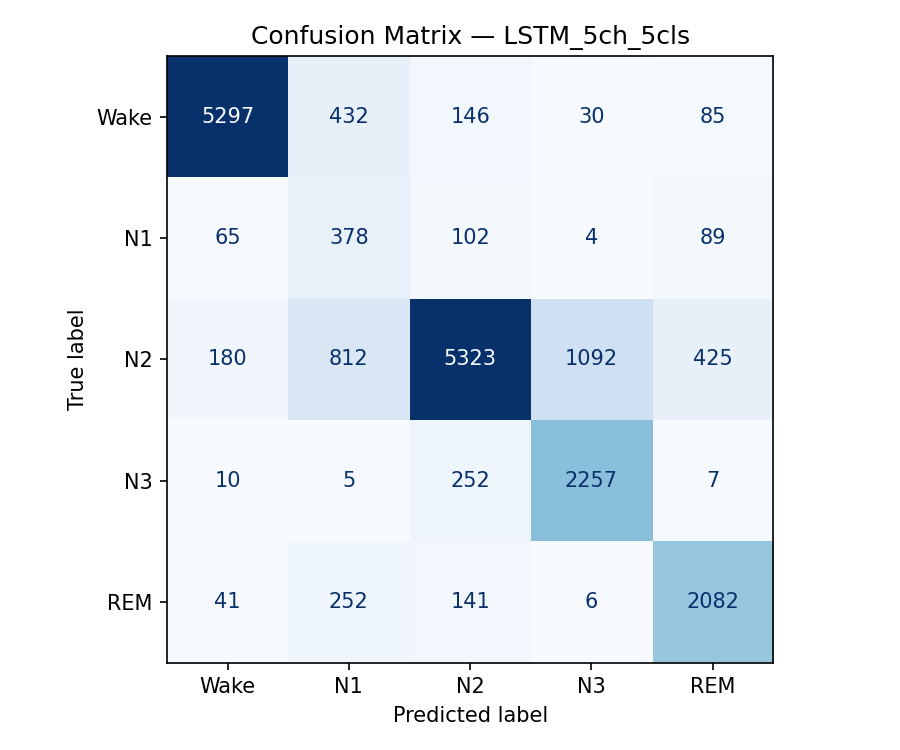
\includegraphics[width=\linewidth]{images/resultats/cm_LSTM_5ch_5cls.png}
  \caption{Récurrent, 5 dérivations}
\end{subfigure}\hfill
\begin{subfigure}[t]{0.48\textwidth}
  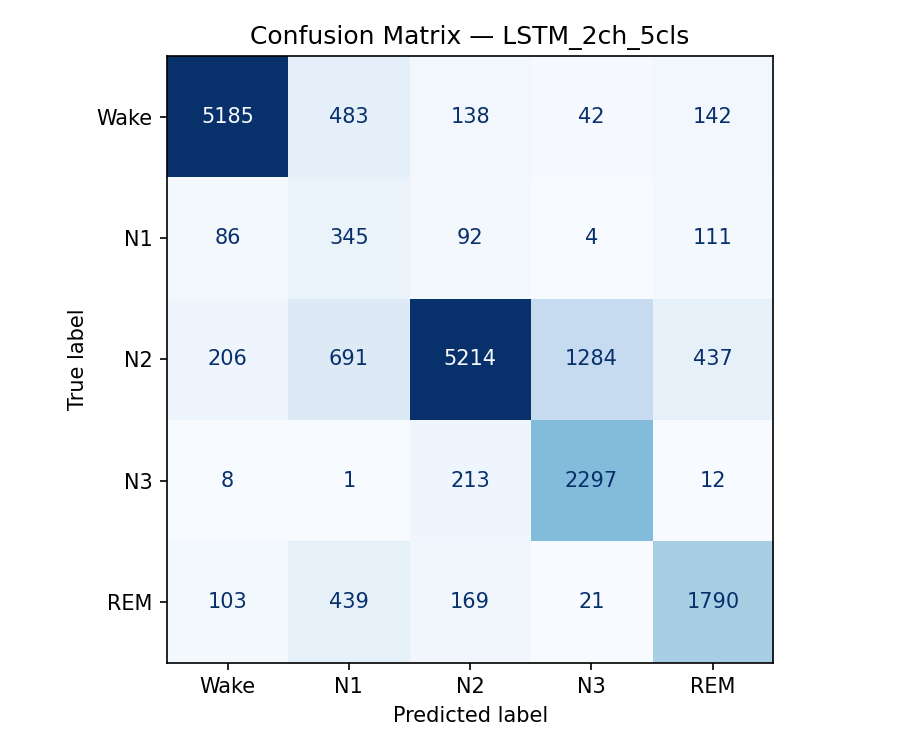
\includegraphics[width=\linewidth]{images/resultats/cm_LSTM_2ch_5cls.png}
  \caption{Récurrent, 2 dérivations}
\end{subfigure}\\[8pt]
\begin{subfigure}[t]{0.48\textwidth}
  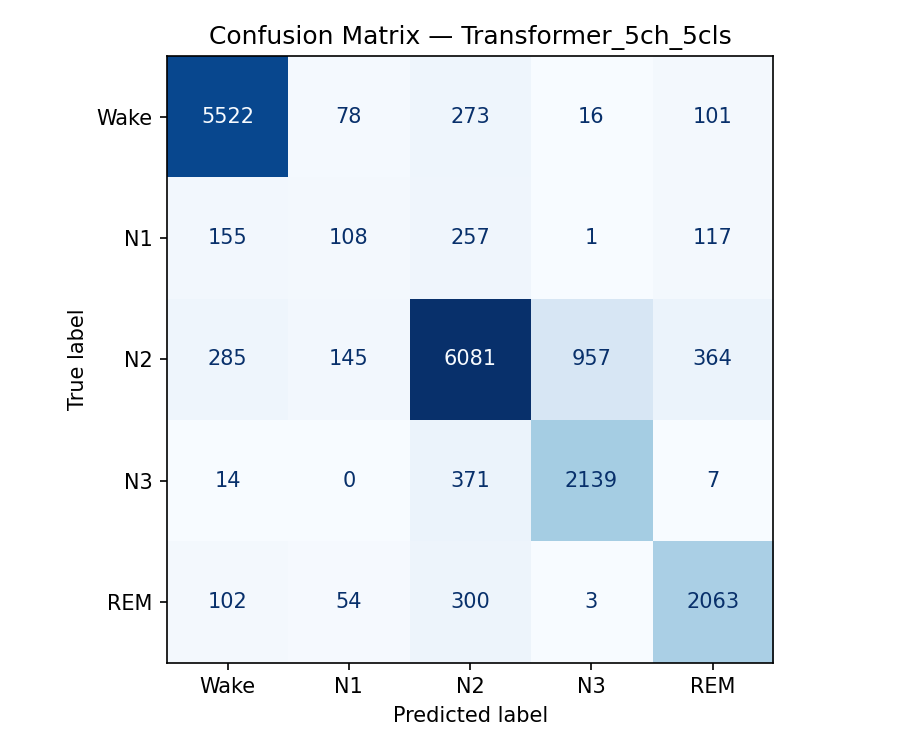
\includegraphics[width=\linewidth]{images/resultats/cm_Transformer_5ch_5cls.png}
  \caption{Attentionnel, 5 dérivations}
\end{subfigure}\hfill
\begin{subfigure}[t]{0.48\textwidth}
  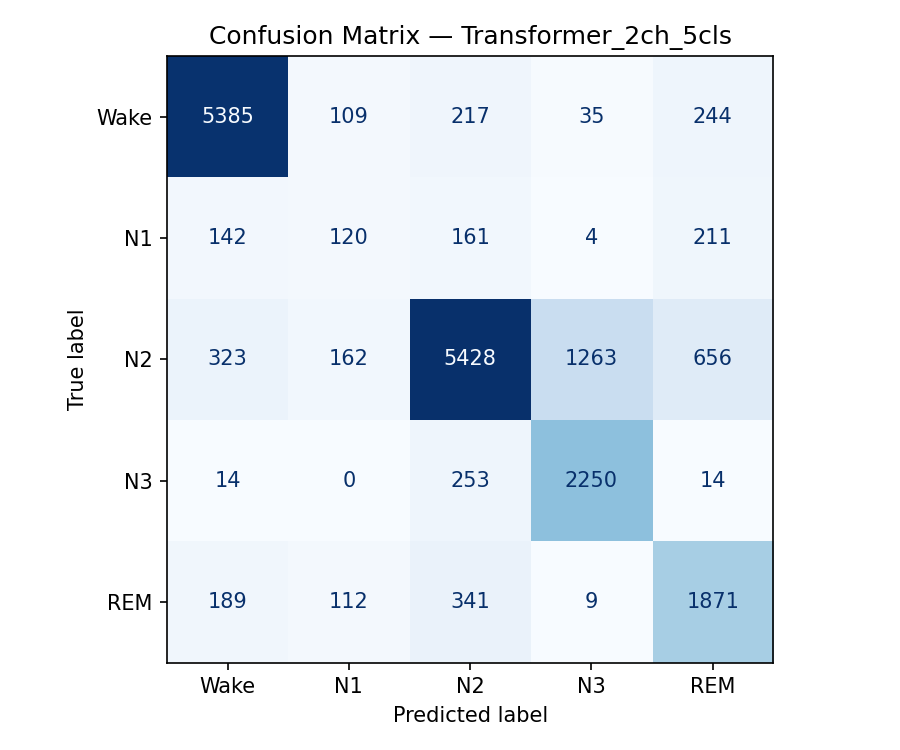
\includegraphics[width=\linewidth]{images/resultats/cm_Transformer_2ch_5cls.png}
  \caption{Attentionnel, 2 dérivations}
\end{subfigure}
\caption[Matrices de confusion --- classification en cinq stades]%
        {Matrices de confusion des six modèles de classification en cinq stades. La
         colonne N1 illustre la difficulté commune aux trois architectures.}
\label{fig:ann-cm-5cls}
\end{figure}

\clearpage
% -----------------------------------------------------------------------------
\section{Ensembles par empilement}
% -----------------------------------------------------------------------------

Pour chaque configuration, la figure de gauche compare les $\kappa$ obtenus par les
trois modèles de base, par le vote moyen et par le méta-apprenant ; celle de droite
donne la matrice de confusion de l'ensemble. Les jeux de test sont ici constitués par
découpage au niveau des sujets et comptent \num{20314} époques.

\begin{figure}[H]
\centering
\begin{subfigure}[t]{0.58\textwidth}
  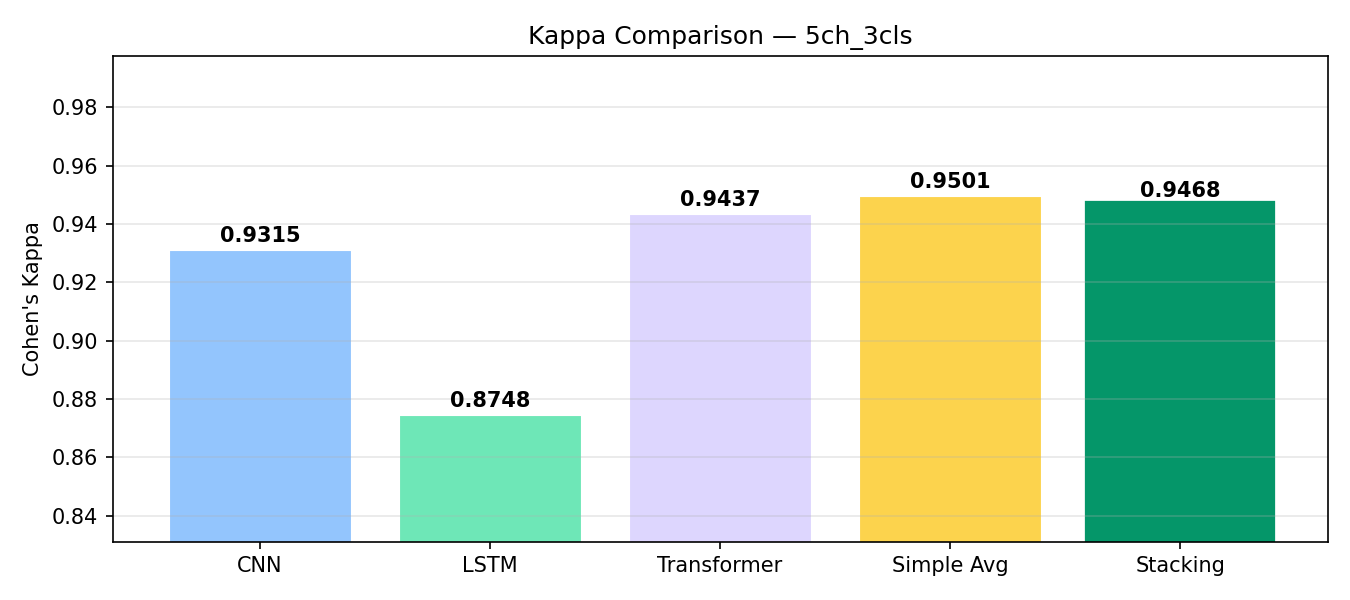
\includegraphics[width=\linewidth]{images/resultats/kappa_comparison_5ch_3cls.png}
  \caption{Comparaison --- 5 dérivations, 3 classes}
\end{subfigure}\hfill
\begin{subfigure}[t]{0.40\textwidth}
  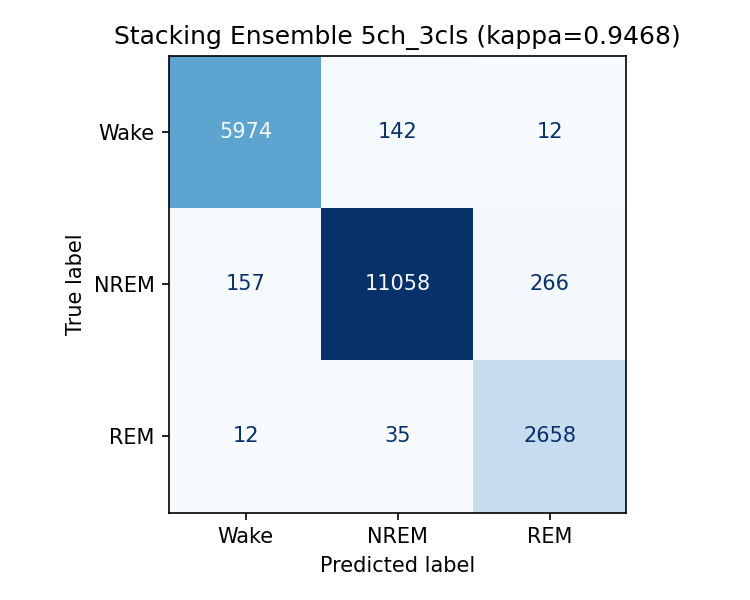
\includegraphics[width=\linewidth]{images/resultats/cm_stacking_5ch_3cls.png}
  \caption{Confusion --- 5 dérivations, 3 classes}
\end{subfigure}\\[8pt]
\begin{subfigure}[t]{0.58\textwidth}
  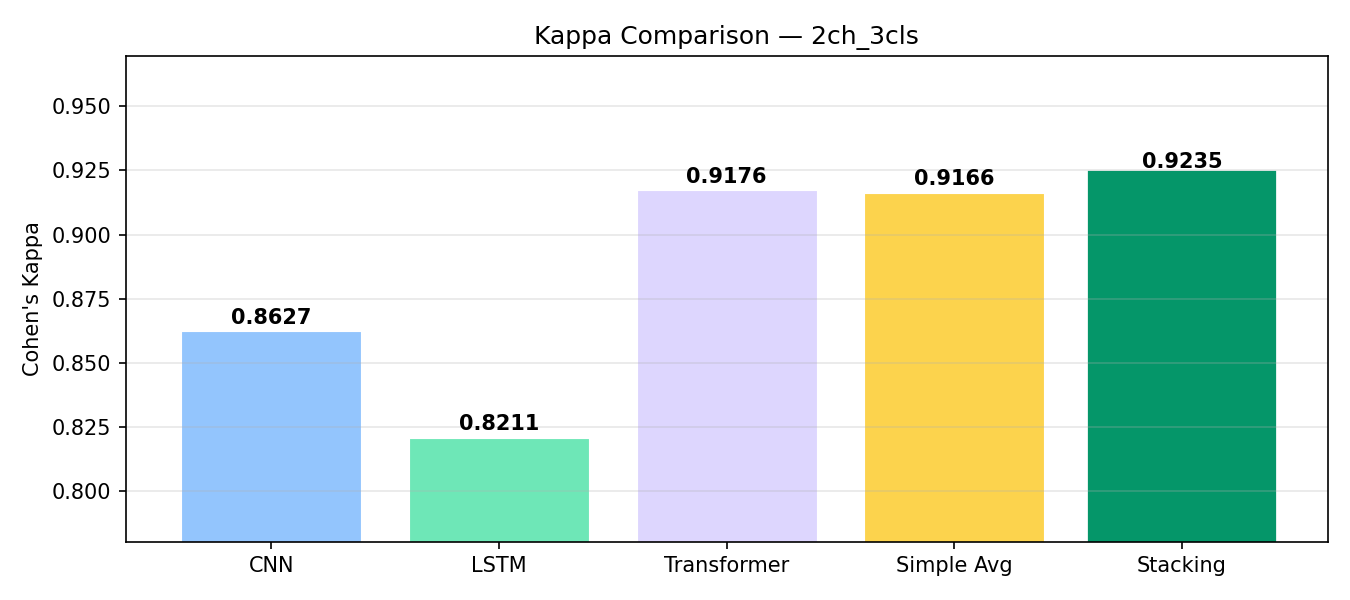
\includegraphics[width=\linewidth]{images/resultats/kappa_comparison_2ch_3cls.png}
  \caption{Comparaison --- 2 dérivations, 3 classes}
\end{subfigure}\hfill
\begin{subfigure}[t]{0.40\textwidth}
  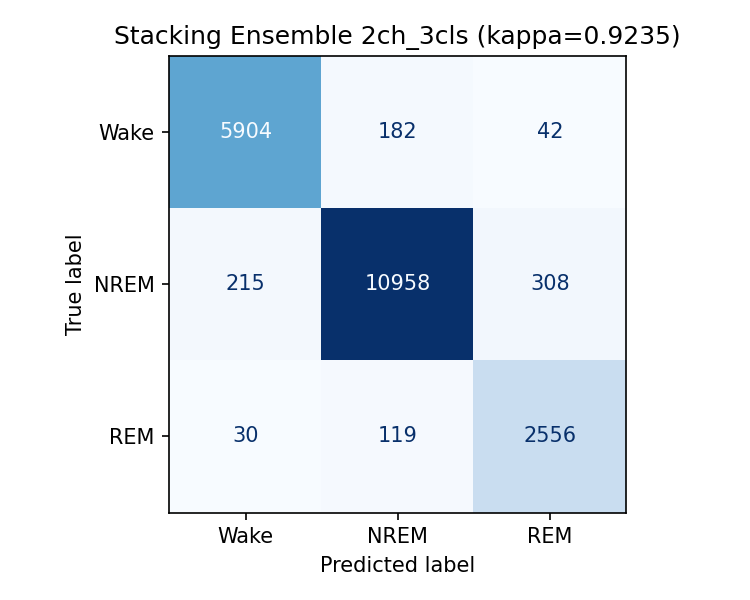
\includegraphics[width=\linewidth]{images/resultats/cm_stacking_2ch_3cls.png}
  \caption{Confusion --- 2 dérivations, 3 classes}
\end{subfigure}\\[8pt]
\begin{subfigure}[t]{0.58\textwidth}
  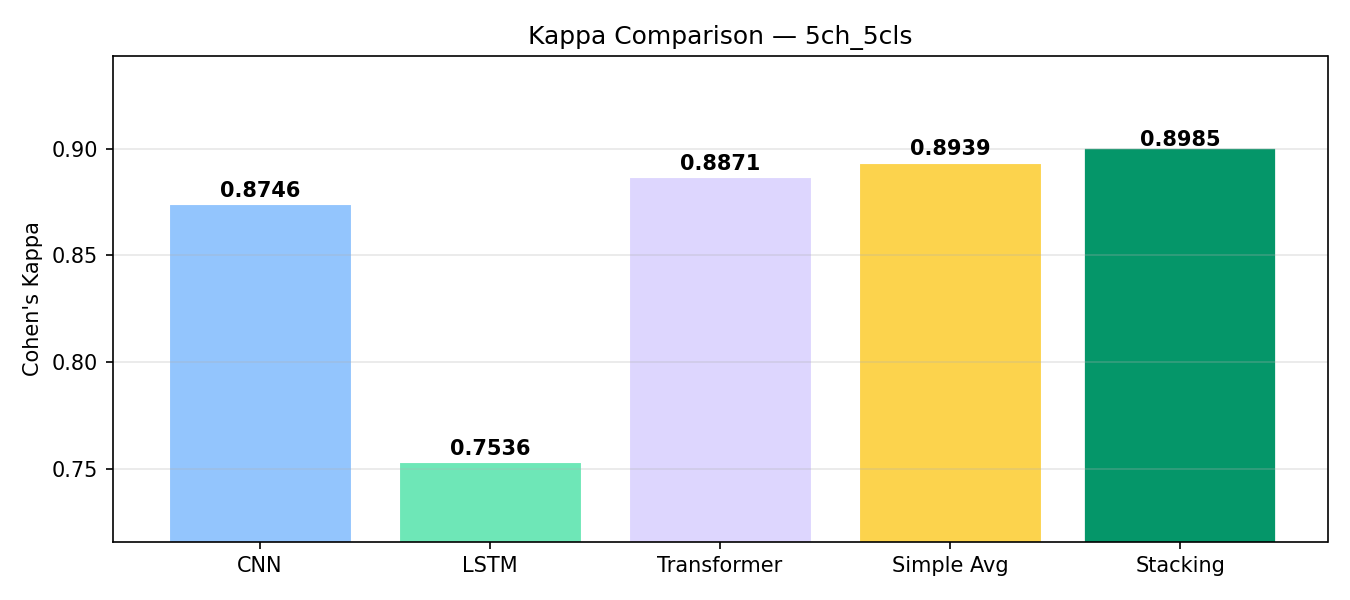
\includegraphics[width=\linewidth]{images/resultats/kappa_comparison_5ch_5cls.png}
  \caption{Comparaison --- 5 dérivations, 5 classes}
\end{subfigure}\hfill
\begin{subfigure}[t]{0.40\textwidth}
  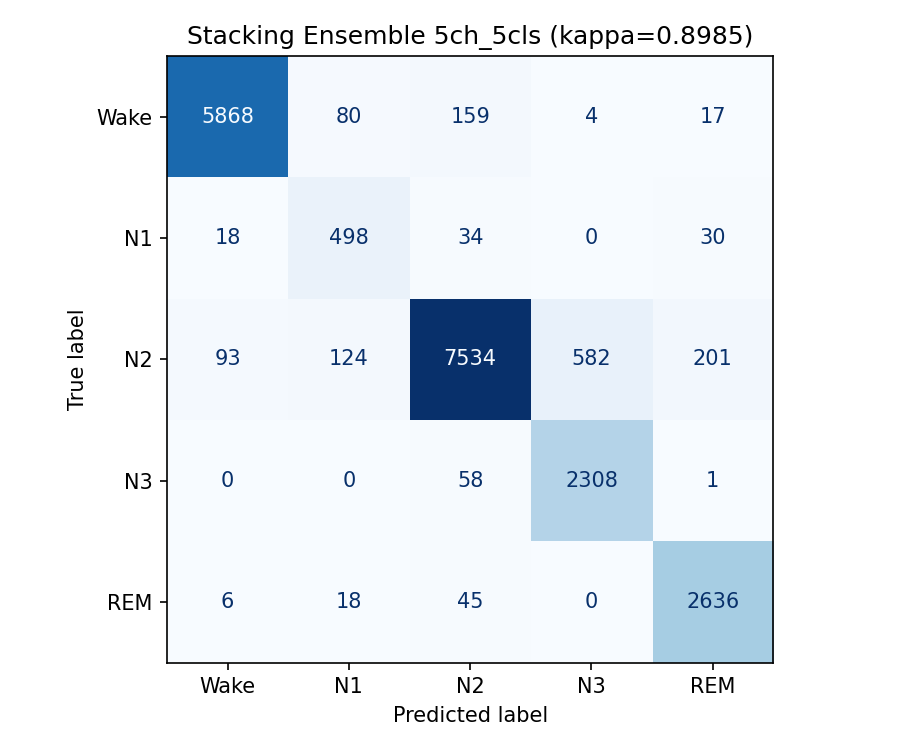
\includegraphics[width=\linewidth]{images/resultats/cm_stacking_5ch_5cls.png}
  \caption{Confusion --- 5 dérivations, 5 classes}
\end{subfigure}\\[8pt]
\begin{subfigure}[t]{0.58\textwidth}
  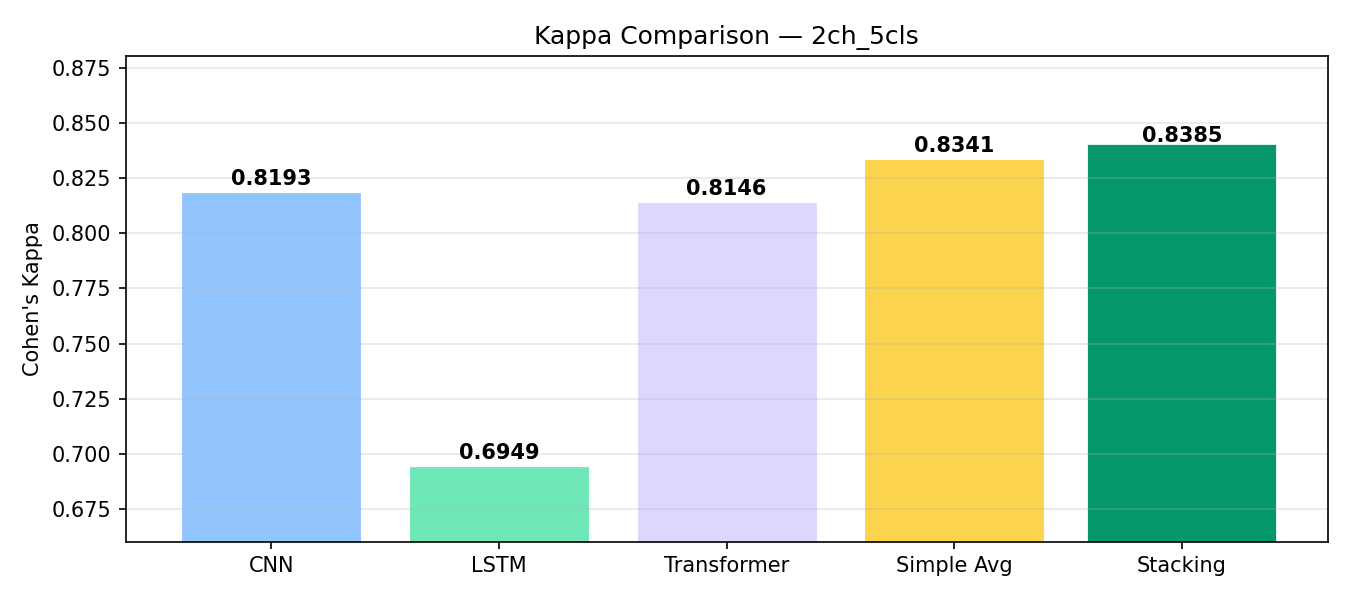
\includegraphics[width=\linewidth]{images/resultats/kappa_comparison_2ch_5cls.png}
  \caption{Comparaison --- 2 dérivations, 5 classes}
\end{subfigure}\hfill
\begin{subfigure}[t]{0.40\textwidth}
  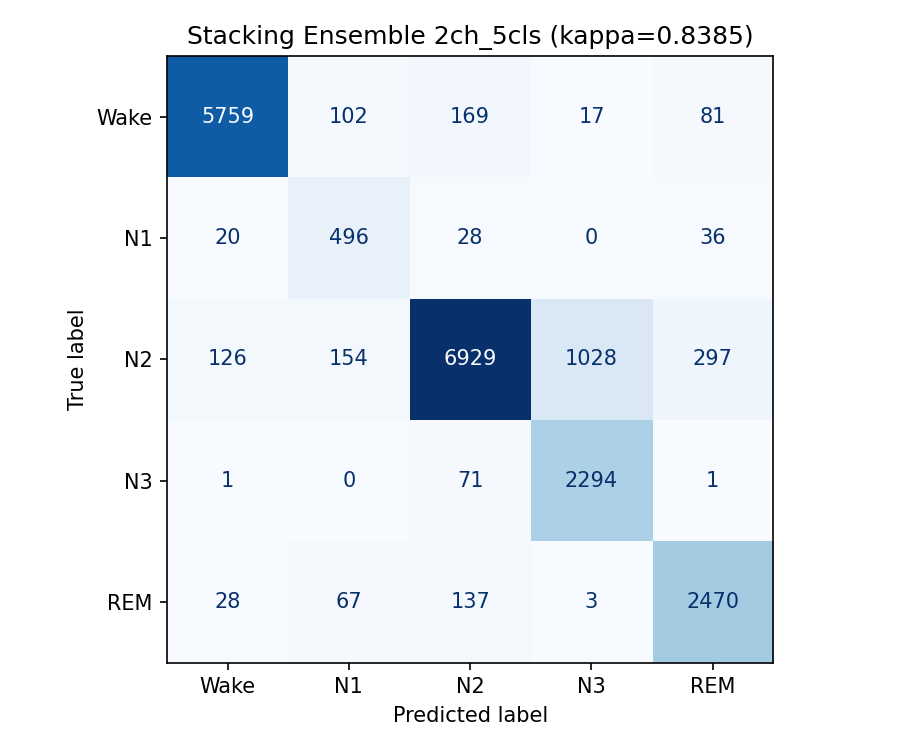
\includegraphics[width=\linewidth]{images/resultats/cm_stacking_2ch_5cls.png}
  \caption{Confusion --- 2 dérivations, 5 classes}
\end{subfigure}
\caption[Résultats des quatre ensembles par empilement]%
        {Résultats des quatre ensembles : comparaison des $\kappa$ et matrices de
         confusion.}
\label{fig:ann-stacking}
\end{figure}

\clearpage
% -----------------------------------------------------------------------------
\section{Rapports de classification détaillés}
% -----------------------------------------------------------------------------

\begin{table}[H]
\centering
\caption{Précision, rappel et F1 par classe --- classification en trois stades}
\label{tab:ann-rapport3}
\small
\begin{tabular}{@{}llccccccccc@{}}
\toprule
& & \multicolumn{3}{c}{\textbf{Éveil}} & \multicolumn{3}{c}{\textbf{NREM}} &
\multicolumn{3}{c}{\textbf{REM}} \\
\cmidrule(lr){3-5}\cmidrule(lr){6-8}\cmidrule(lr){9-11}
\textbf{Dériv.} & \textbf{Architecture} & P & R & F1 & P & R & F1 & P & R & F1 \\
\midrule
\multirow{3}{*}{5}
 & Convolutif   & 0,94 & 0,92 & 0,93 & 0,92 & 0,94 & 0,93 & 0,84 & 0,79 & 0,82 \\
 & Récurrent    & 0,90 & 0,94 & 0,92 & 0,95 & 0,90 & 0,93 & 0,77 & 0,88 & 0,82 \\
 & Attentionnel & 0,92 & 0,91 & 0,91 & 0,92 & 0,92 & 0,92 & 0,79 & 0,77 & 0,78 \\
\midrule
\multirow{3}{*}{2}
 & Convolutif   & 0,88 & 0,93 & 0,90 & 0,92 & 0,91 & 0,92 & 0,78 & 0,72 & 0,75 \\
 & Récurrent    & 0,91 & 0,91 & 0,91 & 0,95 & 0,87 & 0,90 & 0,62 & 0,84 & 0,71 \\
 & Attentionnel & 0,88 & 0,91 & 0,89 & 0,90 & 0,89 & 0,90 & 0,70 & 0,68 & 0,69 \\
\bottomrule
\end{tabular}
\end{table}

\begin{table}[H]
\centering
\caption{F1 par classe --- classification en cinq stades}
\label{tab:ann-rapport5}
\small
\begin{tabular}{@{}llccccc@{}}
\toprule
\textbf{Dériv.} & \textbf{Architecture} & \textbf{Éveil} & \textbf{N1} & \textbf{N2} &
\textbf{N3} & \textbf{REM} \\
\midrule
\multirow{3}{*}{5}
 & Convolutif   & 0,92 & \textcolor{hypnored}{0,26} & 0,82 & 0,78 & 0,82 \\
 & Récurrent    & 0,91 & \textcolor{hypnored}{0,30} & 0,77 & 0,76 & 0,80 \\
 & Attentionnel & 0,92 & \textcolor{hypnored}{0,21} & 0,80 & 0,76 & 0,80 \\
\midrule
\multirow{3}{*}{2}
 & Convolutif   & 0,91 & \textcolor{hypnored}{0,23} & 0,80 & 0,77 & 0,74 \\
 & Récurrent    & 0,90 & \textcolor{hypnored}{0,27} & 0,76 & 0,74 & 0,71 \\
 & Attentionnel & 0,89 & \textcolor{hypnored}{0,21} & 0,76 & 0,74 & 0,68 \\
\bottomrule
\end{tabular}
\end{table}

\begin{table}[H]
\centering
\caption{Rapports de classification des quatre ensembles}
\label{tab:ann-rapport-stack}
\small
\begin{tabular}{@{}lccccccc@{}}
\toprule
\textbf{Configuration} & \textbf{Exactitude} & \textbf{$\kappa$} &
\textbf{F1 macro} & \textbf{F1 pondéré} & \textbf{Effectif} \\
\midrule
5 dérivations, 3 classes & \SI{96,93}{\percent} & 0,947 & 0,96 & 0,97 & \num{20314} \\
2 dérivations, 3 classes & \SI{95,59}{\percent} & 0,924 & 0,95 & 0,96 & \num{20314} \\
5 dérivations, 5 classes & \SI{92,76}{\percent} & 0,899 & 0,90 & 0,93 & \num{20314} \\
2 dérivations, 5 classes & \SI{88,35}{\percent} & 0,839 & 0,84 & 0,89 & \num{20314} \\
\bottomrule
\end{tabular}
\vspace{2pt}
\raggedright\footnotesize
Ces valeurs portent sur un découpage au niveau des sujets et ne sont pas comparables
à celles des modèles de base, évalués sur un découpage au niveau des époques
(voir la discussion des limites, chapitre~\ref{chap:realisation-ia}).
\end{table}

\clearpage
% =============================================================================
\chapter{Résultats détaillés de la prédiction de sévérité}
\label{annexe:osa}
% =============================================================================

\section{Variables du modèle}

Le vecteur d'entrée compte \textbf{53 variables}, réparties en trois familles.

\begin{table}[H]
\centering
\caption{Les 53 variables du modèle de sévérité}
\label{tab:ann-variables}
\small
\begin{tabular}{@{}lcL{9.2cm}@{}}
\toprule
\textbf{Famille} & \textbf{Nombre} & \textbf{Variables} \\
\midrule
Architecture du sommeil\newline\emph{(extraites de l'hypnogramme)} & 25 &
Latence d'endormissement, temps de sommeil total, temps au lit, durée de la période de
sommeil, efficacité, éveil intra-sommeil, proportions de N1, N2, N3 et REM, latences
du REM et du N3, index de fragmentation, nombre et durée moyenne des épisodes d'éveil,
nombre et durée moyenne des épisodes de REM, rapports NREM/REM et léger/profond, six
probabilités de transition \\
\addlinespace[3pt]
Cliniques\newline\emph{(issues de la cohorte)} & 20 &
Saturation moyenne et minimale, proportions de temps sous \SI{95}{\percent},
\SI{90}{\percent} et \SI{85}{\percent}, index d'éveil global, en NREM et en REM,
efficacité et latence de sommeil scorées, proportions de stades scorées, éveil
intra-sommeil, répartition du REM, indice de masse corporelle, âge, sexe \\
\addlinespace[3pt]
Interactions\newline\emph{(construites)} & 8 &
Score d'hypoxie pondéré, éveils $\times$ fragmentation, amplitude de désaturation,
éveils par épisode, rapport des éveils REM/NREM, éveil intra-sommeil $\times$ éveils,
suppression du N3, indice de masse corporelle $\times$ éveils \\
\bottomrule
\end{tabular}
\end{table}

Les index de perturbation respiratoire disponibles dans la cohorte ont été
délibérément écartés : ils mesurent directement les événements dont la sévérité est à
prédire.

\section{Comparaison des classifieurs et résultats}

\begin{figure}[H]
\centering
\begin{subfigure}[t]{0.48\textwidth}
  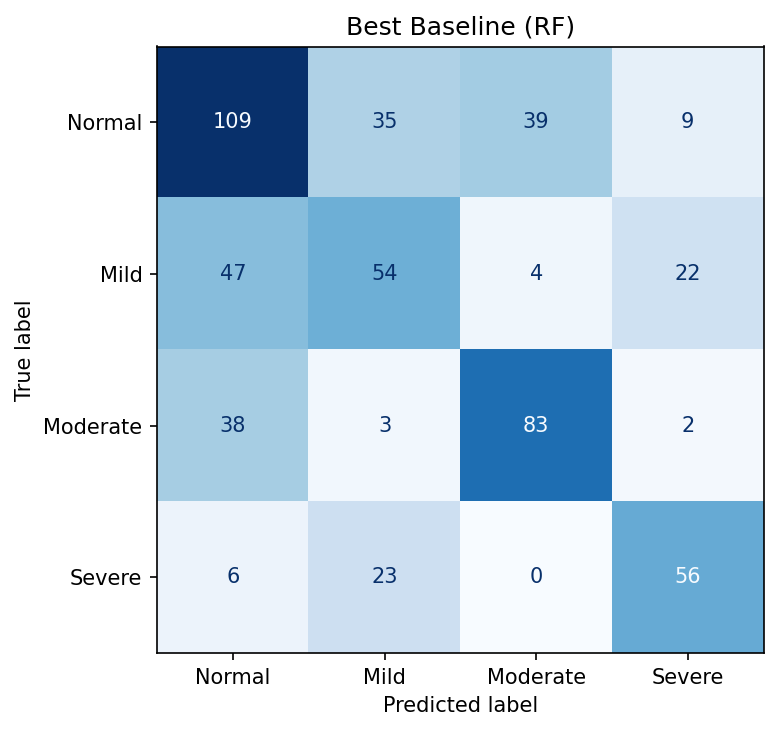
\includegraphics[width=\linewidth]{images/resultats/cm_baseline.png}
  \caption{Meilleure ligne de base --- forêt aléatoire}
\end{subfigure}\hfill
\begin{subfigure}[t]{0.48\textwidth}
  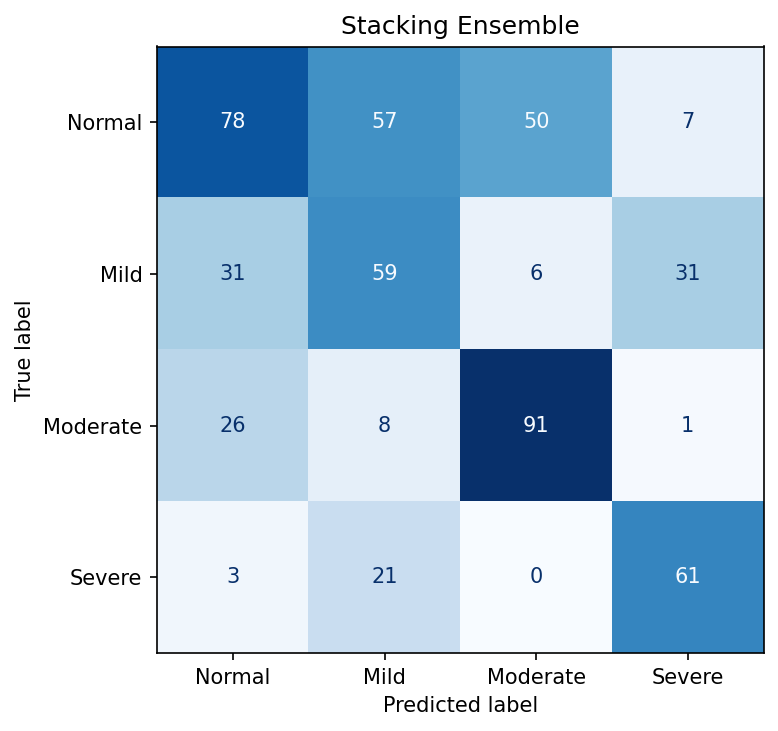
\includegraphics[width=\linewidth]{images/resultats/cm_stacking.png}
  \caption{Ensemble par empilement}
\end{subfigure}
\caption[Matrices de confusion de la prédiction de sévérité]%
        {Matrices de confusion sur les \num{530} sujets de test. \textbf{Attention :}
         ces figures sont celles produites par le script d'origine, dont les
         étiquettes d'axes suivent l'ordre de sévérité alors que l'encodage effectif
         est alphabétique. L'ordre réel des lignes et colonnes est \emph{Léger,
         Modéré, Normal, Sévère}. Les matrices corrigées figurent au
         chapitre~\ref{chap:realisation-ia}.}
\label{fig:ann-cm-osa}
\end{figure}

\begin{table}[H]
\centering
\caption{F1 macro en validation croisée à cinq plis}
\label{tab:ann-cv}
\small
\begin{tabular}{@{}lcc@{}}
\toprule
\textbf{Classifieur} & \textbf{F1 macro} & \textbf{Retenu dans l'ensemble} \\
\midrule
Forêt aléatoire            & 0,558 & oui \\
Gradient boosté (XGBoost)  & 0,552 & oui \\
Gradient boosté (LightGBM) & 0,544 & oui \\
Perceptron multicouche     & 0,522 & non \\
Machine à vecteurs de support & 0,492 & non \\
$k$ plus proches voisins   & 0,456 & non \\
\bottomrule
\end{tabular}
\end{table}

% =============================================================================
\chapter{Dictionnaire de données}
\label{annexe:dico}
% =============================================================================

Cette annexe décrit exhaustivement le schéma relationnel de la plateforme, table par
table et colonne par colonne. Les types indiqués sont ceux du modèle applicatif ; leur
correspondance en base est assurée par la couche de correspondance objet-relationnel.

Conventions : \textbf{CP} désigne une clé primaire, \textbf{CE} une clé étrangère,
\textbf{U} une contrainte d'unicité et \textbf{I} un index. La mention
\emph{obligatoire} signifie que la colonne n'accepte pas de valeur nulle.

% -----------------------------------------------------------------------------
\section{Table \texttt{hospitals}}
% -----------------------------------------------------------------------------

Établissements cliniques auxquels les praticiens sont rattachés.

\begin{table}[H]
\centering
\small
\begin{tabular}{@{}lllL{6.0cm}@{}}
\toprule
\textbf{Colonne} & \textbf{Type} & \textbf{Contrainte} & \textbf{Description} \\
\midrule
\texttt{id}            & entier    & CP, I & Identifiant technique \\
\texttt{name}          & chaîne    & U, I  & Raison sociale de l'établissement \\
\texttt{b2\_bucket}    & chaîne    & ---   & Compartiment de stockage dédié, prévu pour
                                             un cloisonnement par établissement \\
\texttt{billing\_tier} & chaîne    & défaut \texttt{Standard} & Niveau de service
                                             contractuel \\
\texttt{created\_at}   & horodatage& défaut date courante & Date de création de la
                                             fiche \\
\bottomrule
\end{tabular}
\end{table}

% -----------------------------------------------------------------------------
\section{Table \texttt{users}}
% -----------------------------------------------------------------------------

Comptes de la plateforme. Les deux rôles partagent une même table, le champ
\texttt{role} portant la distinction.

\begin{table}[H]
\centering
\small
\begin{tabular}{@{}lllL{5.6cm}@{}}
\toprule
\textbf{Colonne} & \textbf{Type} & \textbf{Contrainte} & \textbf{Description} \\
\midrule
\texttt{id}               & entier     & CP, I & Identifiant technique \\
\texttt{email}            & chaîne     & U, I, obligatoire & Adresse électronique,
                                          servant d'identifiant de connexion \\
\texttt{hashed\_password} & chaîne     & obligatoire & Empreinte bcrypt du mot de
                                          passe, sel inclus \\
\texttt{role}             & chaîne     & défaut \texttt{doctor} & \texttt{admin},
                                          \texttt{doctor} ou \texttt{clinic\_admin} \\
\texttt{first\_name}      & chaîne     & --- & Prénom \\
\texttt{last\_name}       & chaîne     & --- & Nom \\
\texttt{status}           & chaîne     & défaut \texttt{active} & \texttt{active},
                                          \texttt{suspended} ou \texttt{pending} ;
                                          évalué à chaque connexion \\
\texttt{license\_expiry}  & horodatage & --- & Échéance de la licence clinique ;
                                          au-delà, la connexion est refusée \\
\texttt{last\_login}      & horodatage & défaut date courante & Dernière connexion
                                          réussie \\
\texttt{hospital\_id}     & entier     & CE $\to$ \texttt{hospitals.id} &
                                          Établissement de rattachement \\
\bottomrule
\end{tabular}
\end{table}

\noindent
Le rôle \texttt{clinic\_admin} est prévu dans le modèle mais n'est pas exploité par
l'application ; il figure parmi les extensions envisagées.

% -----------------------------------------------------------------------------
\section{Table \texttt{patients}}
% -----------------------------------------------------------------------------

Patients suivis. Le rattachement direct au praticien fonde le cloisonnement des
données : un médecin n'accède qu'aux fiches dont il est le référent.

\begin{table}[H]
\centering
\small
\begin{tabular}{@{}lllL{6.2cm}@{}}
\toprule
\textbf{Colonne} & \textbf{Type} & \textbf{Contrainte} & \textbf{Description} \\
\midrule
\texttt{id}         & entier & CP, I & Identifiant technique \\
\texttt{first\_name}& chaîne & ---   & Prénom \\
\texttt{last\_name} & chaîne & ---   & Nom \\
\texttt{age}        & entier & ---   & Âge en années, variable du modèle de sévérité \\
\texttt{imc}        & réel   & ---   & Indice de masse corporelle, variable du modèle
                                       de sévérité \\
\texttt{gender}     & chaîne & ---   & Sexe, converti en variable binaire à
                                       l'inférence \\
\texttt{doctor\_id} & entier & CE $\to$ \texttt{users.id} & Praticien référent \\
\bottomrule
\end{tabular}
\end{table}

% -----------------------------------------------------------------------------
\section{Table \texttt{psgs}}
% -----------------------------------------------------------------------------

Examens polysomnographiques. Entité pivot du modèle : elle ne stocke que des
\emph{références} vers les fichiers, jamais leur contenu. Ces références sont
converties en liens signés temporaires au moment de composer la réponse.

\begin{table}[H]
\centering
\small
\begin{tabular}{@{}lllL{5.4cm}@{}}
\toprule
\textbf{Colonne} & \textbf{Type} & \textbf{Contrainte} & \textbf{Description} \\
\midrule
\texttt{id}          & entier     & CP, I & Identifiant technique \\
\texttt{patient\_id} & entier     & CE $\to$ \texttt{patients.id} & Patient examiné \\
\texttt{date}        & horodatage & défaut date courante & Date de l'examen \\
\texttt{severity}    & chaîne     & --- & Classe de sévérité prédite \\
\texttt{report\_data}& chaîne     & --- & Document sérialisé des résultats d'analyse :
                                          stades, métriques, marqueurs \\
\texttt{edf\_url}    & chaîne     & --- & Référence de l'enregistrement brut archivé \\
\texttt{hypnogram\_url} & chaîne  & --- & Référence de l'hypnogramme \\
\texttt{hypnogram\_annotated\_url} & chaîne & --- & Référence de l'hypnogramme portant
                                          les annotations du praticien \\
\texttt{csv\_url}    & chaîne     & --- & Référence de l'export tabulaire des
                                          marqueurs \\
\texttt{osa\_report\_url} & chaîne& --- & Référence du compte rendu clinique \\
\bottomrule
\end{tabular}
\end{table}

\noindent
Le champ \texttt{report\_data} est volontairement conservé sous forme sérialisée
plutôt que décomposé en colonnes. La structure des résultats a évolué au fil des
sprints — ajout de la saturation, de la densité d'événements, des comparaisons
normatives — et une décomposition rigide aurait imposé une migration à chaque
évolution. Cette souplesse a un prix : les résultats ne sont pas interrogeables par
requête, ce qu'une version ultérieure devrait corriger pour les métriques les plus
consultées.

% -----------------------------------------------------------------------------
\section{Table \texttt{psg\_annotations}}
% -----------------------------------------------------------------------------

Observations horodatées portées par le praticien sur une époque précise.

\begin{table}[H]
\centering
\small
\begin{tabular}{@{}lllL{6.0cm}@{}}
\toprule
\textbf{Colonne} & \textbf{Type} & \textbf{Contrainte} & \textbf{Description} \\
\midrule
\texttt{id}          & entier     & CP, I & Identifiant technique \\
\texttt{psg\_id}     & entier     & CE $\to$ \texttt{psgs.id} & Examen concerné ;
                                             suppression en cascade \\
\texttt{epoch\_index}& entier     & --- & Rang de l'époque annotée, à partir de zéro \\
\texttt{note}        & chaîne     & --- & Texte libre de l'observation \\
\texttt{created\_at} & horodatage & défaut date courante & Date de saisie \\
\bottomrule
\end{tabular}
\end{table}

% -----------------------------------------------------------------------------
\section{Table \texttt{audit\_logs}}
% -----------------------------------------------------------------------------

Journal de traçabilité. Cette table est \textbf{volontairement dénormalisée} : elle
recopie l'adresse et le rôle de l'auteur au lieu de référencer son compte, afin que la
trace survive à la suppression de celui-ci. Une clé étrangère l'en empêcherait.

\begin{table}[H]
\centering
\small
\begin{tabular}{@{}lllL{6.0cm}@{}}
\toprule
\textbf{Colonne} & \textbf{Type} & \textbf{Contrainte} & \textbf{Description} \\
\midrule
\texttt{id}          & entier     & CP, I & Identifiant technique \\
\texttt{timestamp}   & horodatage & défaut date courante & Instant de l'action \\
\texttt{user\_email} & chaîne     & I & Adresse de l'auteur, recopiée \\
\texttt{user\_role}  & chaîne     & --- & Rôle de l'auteur au moment de l'action \\
\texttt{action}      & chaîne     & --- & Description en clair de l'action \\
\texttt{ip\_address} & chaîne     & --- & Adresse d'origine de la requête \\
\bottomrule
\end{tabular}
\end{table}

\noindent
Sont journalisées les connexions, les créations de compte médecin, les modifications de
statut ou d'échéance de licence et les réinitialisations de mot de passe.

% -----------------------------------------------------------------------------
\section{Table \texttt{file\_conversations}}
% -----------------------------------------------------------------------------

Fils de discussion rattachés à un examen et à exactement deux praticiens.

\begin{table}[H]
\centering
\small
\begin{tabular}{@{}lllL{5.5cm}@{}}
\toprule
\textbf{Colonne} & \textbf{Type} & \textbf{Contrainte} & \textbf{Description} \\
\midrule
\texttt{id}              & entier     & CP, I & Identifiant technique \\
\texttt{psg\_id}         & entier     & CE $\to$ \texttt{psgs.id} & Examen support de
                                                 la discussion \\
\texttt{file\_type}      & chaîne     & --- & Pièce concernée : \texttt{edf},
                                        \texttt{hypnogram}, \texttt{csv} ou
                                        \texttt{xml} \\
\texttt{doctor\_one\_id} & entier     & CE $\to$ \texttt{users.id} & Praticien à
                                                 l'origine de la sollicitation \\
\texttt{doctor\_two\_id} & entier     & CE $\to$ \texttt{users.id} & Confrère sollicité \\
\texttt{created\_at}     & horodatage & défaut date courante & Date d'ouverture \\
\bottomrule
\end{tabular}
\end{table}

% -----------------------------------------------------------------------------
\section{Table \texttt{file\_messages}}
% -----------------------------------------------------------------------------

Messages échangés au sein d'un fil.

\begin{table}[H]
\centering
\small
\begin{tabular}{@{}lllL{5.8cm}@{}}
\toprule
\textbf{Colonne} & \textbf{Type} & \textbf{Contrainte} & \textbf{Description} \\
\midrule
\texttt{id}               & entier     & CP, I & Identifiant technique \\
\texttt{conversation\_id} & entier     & CE $\to$ \texttt{file\_conversations.id} &
                                          Fil concerné ; suppression en cascade \\
\texttt{sender\_id}       & entier     & CE $\to$ \texttt{users.id} & Auteur du
                                          message \\
\texttt{content}          & chaîne     & --- & Corps du message \\
\texttt{timestamp}        & horodatage & défaut date courante & Instant d'émission \\
\bottomrule
\end{tabular}
\end{table}

% -----------------------------------------------------------------------------
\section{Synthèse des relations}
% -----------------------------------------------------------------------------

\begin{table}[H]
\centering
\caption{Relations entre les tables}
\label{tab:ann-relations}
\small
\begin{tabular}{@{}llcL{5.4cm}@{}}
\toprule
\textbf{Depuis} & \textbf{Vers} & \textbf{Cardinalité} & \textbf{Sémantique} \\
\midrule
\texttt{hospitals} & \texttt{users}    & 1 -- 0..* & Un établissement emploie
                                                     plusieurs praticiens \\
\texttt{users}     & \texttt{patients} & 1 -- 0..* & Un praticien suit plusieurs
                                                     patients \\
\texttt{patients}  & \texttt{psgs}     & 1 -- 0..* & Un patient peut subir plusieurs
                                                     examens \\
\texttt{psgs}      & \texttt{psg\_annotations} & 1 -- 0..* & Un examen porte plusieurs
                                                     annotations \\
\texttt{psgs}      & \texttt{file\_conversations} & 1 -- 0..* & Un examen peut susciter
                                                     plusieurs discussions \\
\texttt{users}     & \texttt{file\_conversations} & 2 -- 0..* & Chaque discussion
                                                     réunit exactement deux praticiens \\
\texttt{file\_conversations} & \texttt{file\_messages} & 1 -- 0..* & Un fil contient
                                                     plusieurs messages \\
\texttt{users}     & \texttt{file\_messages} & 1 -- 0..* & Un praticien émet plusieurs
                                                     messages \\
\bottomrule
\end{tabular}
\end{table}

Les suppressions en cascade sont déclarées sur deux relations seulement : celle qui lie
un examen à ses annotations, et celle qui lie un fil à ses messages. Partout ailleurs,
la suppression d'un parent est volontairement bloquée par l'intégrité référentielle :
sur un système hébergeant des dossiers médicaux, une suppression accidentelle en
cascade serait irrattrapable.

% =============================================================================
\chapter{Manuel utilisateur}
\label{annexe:manuel}
% =============================================================================

Ce manuel décrit les parcours des deux profils d'utilisateur. Il suppose la plateforme
déjà déployée ; les modalités de déploiement figurent au
chapitre~\ref{chap:realisation-plateforme}.

% -----------------------------------------------------------------------------
\section{Premiers pas}
% -----------------------------------------------------------------------------

\subsection*{Se connecter}

La page d'accueil publique présente la plateforme et donne accès au formulaire de
connexion. Saisissez votre adresse électronique et votre mot de passe.

Trois refus sont possibles, chacun accompagné d'un message distinct. Un
\emph{identifiant ou mot de passe incorrect} signale une erreur de saisie. Un
\emph{compte suspendu} ou \emph{en attente d'approbation} impose de contacter votre
administrateur. Une \emph{licence expirée} impose de la renouveler auprès de lui.

Votre session reste ouverte sept jours. Le bouton de déconnexion figure au bas du menu
latéral.

\subsection*{Régler l'affichage}

Deux réglages sont disponibles au bas du menu latéral : la \textbf{langue}, qui bascule
immédiatement entre le français et l'anglais, et le \textbf{thème sombre}, adapté à la
lecture prolongée en faible luminosité.

% -----------------------------------------------------------------------------
\section{Profil médecin}
% -----------------------------------------------------------------------------

\subsection*{Tableau de bord}

À la connexion, le tableau de bord présente le nombre de patients suivis, le nombre
d'examens réalisés, le nombre de risques sévères détectés, la répartition des risques
d'apnée sur votre patientèle et la liste de vos derniers patients.

\subsection*{Enregistrer un patient}

Ouvrez \textbf{Mes patients}, puis \textbf{Nouveau patient}. Renseignez le nom complet,
l'âge, l'indice de masse corporelle et le sexe.

Ces trois dernières valeurs ne sont pas administratives : elles alimentent directement
le modèle de prédiction de sévérité. Un indice de masse corporelle erroné dégradera
l'estimation du risque.

\subsection*{Analyser un enregistrement}

Le parcours d'analyse se déroule en quatre étapes.

\begin{enumerate}[itemsep=3pt,topsep=4pt]
  \item \textbf{Déclarer le montage.} Choisissez \emph{5 canaux} si l'enregistrement
        comporte les deux dérivations électroencéphalographiques, les deux
        électro-oculogrammes et l'électromyogramme mentonnier ; c'est le montage
        clinique complet et le plus précis. Choisissez \emph{2 canaux} pour un
        enregistrement ambulatoire limité aux dérivations
        électroencéphalographiques.
  \item \textbf{Choisir la granularité.} \emph{3 classes} — éveil, sommeil lent,
        sommeil paradoxal — est le réglage recommandé : il est nettement plus robuste
        et suffit à l'évaluation du risque d'apnée. \emph{5 classes} restitue les
        stades N1, N2 et N3 séparément, au prix d'une précision moindre, notamment sur
        le stade N1.
  \item \textbf{Déposer le fichier.} Glissez l'enregistrement au format EDF dans la
        zone prévue, ou cliquez pour le sélectionner. Un récapitulatif rappelle vos
        choix avant lancement.
  \item \textbf{Consulter les résultats.} L'écran de progression détaille les étapes du
        traitement. Comptez quelques dizaines de secondes pour une nuit complète.
\end{enumerate}

\noindent
Si une dérivation attendue est absente du fichier, le système applique un repli
documenté sur la dérivation électroencéphalographique principale et poursuit l'analyse.
La précision s'en trouve réduite : vérifiez le montage réel avant d'interpréter.

\subsection*{Lire les résultats}

La page de résultats se lit de haut en bas.

Le \textbf{graphique intégré} superpose sur un même axe temporel l'hypnogramme prédit,
la densité d'événements respiratoires et la courbe de saturation. C'est la vue la plus
informative : elle permet de constater directement qu'une désaturation coïncide avec un
épisode particulier.

Les \textbf{métriques AASM} sont présentées en cartes : efficacité du sommeil, temps de
sommeil total, temps passé au lit, latence d'endormissement, latence du sommeil
paradoxal et durée d'éveil intra-sommeil. Chacune indique sa plage de référence et sa
position par rapport aux valeurs de la cohorte de référence. Une valeur hors norme est
signalée.

Les \textbf{alertes cliniques} reprennent en clair les anomalies détectées : efficacité
insuffisante, sommeil paradoxal réduit, fragmentation excessive.

Les \textbf{marqueurs extraits} détaillent la temporalité, la distribution des stades,
les latences, la fragmentation et la répartition du sommeil paradoxal. Ils sont
exportables au format tabulaire ou balisé.

\subsection*{Annoter l'hypnogramme}

Cliquez sur le graphique pour annoter une époque. Vos observations sont conservées et
peuvent être synchronisées vers le dossier de l'examen, ce qui archive l'hypnogramme
annoté aux côtés des autres pièces.

\subsection*{Évaluer le risque d'apnée}

Sous les résultats, complétez le formulaire clinique : données démographiques et
oxymétrie nocturne. Les index de micro-éveils sont facultatifs mais améliorent la
précision. Les champs laissés vides sont comblés par la valeur médiane de la population
de référence, ce que le rapport signale.

Le résultat comprend la \textbf{classe de sévérité}, ses \textbf{probabilités} et les
\textbf{facteurs déterminants}, présentés en deux colonnes : ce qui aggrave
l'estimation et ce qui la tempère.

\begin{samepage}
\noindent\textbf{Comment interpréter les facteurs.} Ils décrivent le raisonnement du
\emph{modèle}, non une causalité physiologique. Un facteur fortement contributif
signale une variable qui a pesé sur la prédiction ; il n'établit pas que cette variable
cause le trouble. La décision diagnostique vous revient.
\end{samepage}

\subsection*{Prédire sans enregistrement}

L'entrée \textbf{OSA Custom} permet une estimation sans fichier EDF, à partir d'un
compte rendu produit ailleurs. Deux voies sont offertes : la saisie manuelle des
marqueurs, ou l'import d'un fichier tabulaire ou balisé qui préremplit automatiquement
le formulaire.

\subsection*{Produire le compte rendu}

Le bouton de téléchargement ouvre un sélecteur de sections : hypnogramme, métriques
AASM, sévérité, facteurs explicatifs, tracés bruts et comparaison aux normes. Ne
retenez que ce qui est pertinent pour le destinataire. Le document produit est archivé
avec l'examen.

\subsection*{Solliciter un confrère}

Depuis la fiche d'un patient, le bouton \textbf{Collaborer} ouvre un fil de discussion
rattaché à l'examen. Sélectionnez le praticien et rédigez votre demande. L'entrée
\textbf{Avis confraternels} rassemble tous vos échanges en cours.

L'intérêt de ce dispositif est que la discussion reste attachée à l'examen : votre
correspondant dispose du contexte sans que vous ayez à le lui transmettre.

% -----------------------------------------------------------------------------
\section{Profil administrateur}
% -----------------------------------------------------------------------------

\subsection*{Créer un compte médecin}

Depuis \textbf{Médecins}, puis \textbf{Nouveau médecin}, renseignez l'identité,
l'adresse électronique, le mot de passe initial, l'établissement de rattachement et
l'échéance de licence.

\subsection*{Gérer le cycle de vie}

Trois opérations sont disponibles sur chaque compte. La \textbf{suspension} bloque
l'accès sans supprimer aucune donnée, et se lève à tout moment. La \textbf{modification
de l'échéance} renouvelle ou raccourcit la licence. La \textbf{réinitialisation du mot
de passe} génère un mot de passe temporaire à transmettre au praticien.

\noindent
Ne supprimez jamais un compte pour retirer un accès : la suspension y pourvoit sans
rompre le lien avec les dossiers patients dont ce praticien est référent.

\subsection*{Gérer les établissements}

L'entrée \textbf{Hôpitaux} permet de déclarer les structures cliniques et de leur
associer un niveau de service. Un praticien rattaché à un établissement en hérite les
paramètres.

\subsection*{Consulter le journal d'audit}

L'entrée \textbf{Journal d'audit} donne accès à la trace de toutes les actions
sensibles : connexions, créations de compte, modifications de statut,
réinitialisations. Chaque entrée porte son auteur, son horodatage et son adresse
d'origine. Le journal est exportable au format tabulaire pour un contrôle externe.

% -----------------------------------------------------------------------------
\section{Questions fréquentes}
% -----------------------------------------------------------------------------

\begin{table}[H]
\centering
\small
\begin{tabular}{@{}L{5.3cm}L{8.8cm}@{}}
\toprule
\textbf{Situation} & \textbf{Conduite à tenir} \\
\midrule
Le dépôt du fichier est refusé &
Seul le format EDF est accepté. Vérifiez l'extension et l'intégrité du fichier. \\
\addlinespace[3pt]
L'analyse échoue immédiatement &
L'enregistrement est probablement plus court qu'une époque de trente secondes, ou ne
contient aucune dérivation électroencéphalographique exploitable. \\
\addlinespace[3pt]
Une vignette signale un échec de transfert &
Les résultats restent consultables : ils sont enregistrés indépendamment du fichier.
Seul l'archivage de l'enregistrement brut a échoué. \\
\addlinespace[3pt]
Un lien vers un fichier ne fonctionne plus &
Les liens expirent au bout de vingt-quatre heures. Rechargez la fiche du patient pour
en obtenir un nouveau. \\
\addlinespace[3pt]
La proportion de N1 semble aberrante &
En classification à trois classes, les proportions de N1, N2 et N3 sont estimées à
partir de ratios de population et non mesurées. Utilisez la granularité à cinq classes
si ces valeurs importent. \\
\addlinespace[3pt]
La connexion est refusée alors que le mot de passe est correct &
Votre compte est suspendu ou votre licence a expiré. Le message précise le cas.
Contactez votre administrateur. \\
\bottomrule
\end{tabular}
\end{table}
